%%%%%%%%%%%%%%%%%%%%%%%%%%%%%%%%%%%%%%%%%%%%%%%%%%%%%%%%%%%%%%%%%%%%%%%
%% P2A manuscript for IJAIT (World Scientific, ws-ijait 2024-10-10)
%% Honest ablation. Do not claim Reliable / contamination / pair-SOTA.
%%%%%%%%%%%%%%%%%%%%%%%%%%%%%%%%%%%%%%%%%%%%%%%%%%%%%%%%%%%%%%%%%%%%%%%
\documentclass{ws-ijait}

\usepackage{xcolor}
\usepackage{tikz}
\usetikzlibrary{arrows.meta,positioning,calc}
\usepackage{algorithm}
\usepackage{algpseudocode}
\usepackage[sort,compress]{cite}
\usepackage{hyperref}
\hypersetup{colorlinks=false,allbordercolors=blue,pdfborderstyle={/S/U/W 1}}

\newcommand{\phat}{\hat{p}}
\newcommand{\chat}{\hat{c}}
\newcommand{\Lirr}{L_{\mathrm{irr}}}

\begin{document}

\markboth{T.\ Do Thi, T.\ Dao Minh and A.-H.\ Dao}
{From Pair Scores to Prerequisite Graphs on Skill-Taxonomy Descriptions}

\catchline{}{}{}{}{}

\title{From Pair Scores to Prerequisite Graphs\\
on Skill-Taxonomy Descriptions:\\
Evidence Format, Lexical Priors, and Graph Constraints}

\author{Thu Do Thi}

\address{Hung Yen University of Technology and Engineering\footnote{Formerly Hung Yen University of Technology and Education; renamed 3 September 2026.},
Hung Yen, Vietnam\\
thudt@utehy.edu.vn}

\author{Tuan Dao Minh}

\address{Hung Yen University of Technology and Engineering,
Hung Yen, Vietnam\\
tuanymc@utehy.edu.vn}

\author{Anh-Hien Dao\footnote{Corresponding author.}}

\address{Hung Yen University of Technology and Engineering,
Hung Yen, Vietnam\\
hienda@utehy.edu.vn}

\maketitle

\begin{history}
\received{(Day Month Year)}
\accepted{(Day Month Year)}
\published{(Day Month Year)}
\end{history}

\begin{abstract}
Prerequisite graphs support curriculum design and skill-based
learning paths, yet language-model predictors usually stop at a
pairwise score that cannot be audited as a graph.
We describe a seven-step tool that turns those scores into a
directed acyclic graph whose edges carry a verbatim skill-card
span.
On the public {ESCO-PrereqSkill} release, under an unseen-concept
split, we separate prompt format, a lexical mention rule,
temperature scaling, and cycle constraints for
\texttt{gpt-4o-mini} and {Qwen} 2.5 7B.
Presenting the skill card as evidence improves ranking for
\texttt{gpt-4o-mini} ({ROC}-{AUC} $0.886$) and lowers it for
{Qwen}.
A mention rule remains the strongest standalone ranker; stacking
it with the model scores, fit on the training pairs, reaches
{PR}-{AUC} $0.260$.
The same constraints then yield two graphs: a higher-recall graph
from the taxonomy prompt (graph {F1} $0.124$) and a
higher-precision graph from the stack (graph {F1} $0.198$).
On taxonomy-derived gold, a lexical rule is a strong prior, and
the language model is most useful as a complementary re-ranker.
\end{abstract}

\keywords{Prerequisite graph; large language models; skill taxonomy;
verbalized confidence; calibration; directed acyclic graph.}

\section{Introduction}
A prerequisite relation specifies which competence must be acquired
before another can be taught or assessed.
Curriculum designers, maintainers of a skill classification such as
{ESCO}, and learning-path recommenders need that relation as an
edge they can inspect: a direction, a span of source text, and a
place in an acyclic graph.
Recent pairwise predictors, including {LECDPR}\cite{Xiao_2026} and
{ProPRL}\cite{Cheng_2026}, optimize a binary label and stop at a
score.
{AutoPRE}\cite{Li_AutoPRE_2025} and {KnowLP}\cite{Cheng_KnowLP}
already use large language models ({LLMs}) for concept
prerequisites.
A score still leaves reverse conflicts and cycles unresolved, so it
is not yet a graph a practitioner can audit.

We study that conversion on skill-taxonomy descriptions.
The aim is diagnostic: each stage is isolated so that its
contribution is visible.
Three questions organize the paper.
\begin{itemize}
\item \textbf{RQ1.} Does presenting a taxonomy description as
evidence improve pairwise ranking, and does the effect depend on
the model?
\item \textbf{RQ2.} Can {LLM} scores add value beyond a lexical
mention rule?
\item \textbf{RQ3.} What do temperature scaling and structural
constraints contribute once those scores are turned into a graph?
\end{itemize}

The contributions answer those questions at the level of the tool.
\begin{romanlist}[(iii)]
\item A seven-step induction procedure whose output edge carries
evidence, a verbalized score, a direction, and a type, together
with an explicit map from each reported metric to the score field
it uses.
\item An ablation of prompt format against a mention rule and a
logistic stack, on an unseen-concept split of
{ESCO-PrereqSkill}\cite{Le_2025}.
\item Two acyclic graphs from the same constraints: one induced
from the taxonomy prompt, and one from the stack.
The first recovers more gold edges; the second is the
higher-precision output.
\end{romanlist}
Presenting the skill card as evidence raises pairwise ranking for
\texttt{gpt-4o-mini} and lowers it for {Qwen} 2.5 7B.
A mention rule is the strongest standalone ranker, and a stack of
that rule with the model scores, fit on the training pairs, reaches
{PR}-{AUC} $0.260$.
The same structural constraints then yield a higher-recall taxonomy
graph and a higher-precision stack graph.
Section~\ref{sec:related} places the tool among pairwise predictors,
taxonomy induction, and verbalized confidence.
Section~\ref{sec:problem} defines the edge.
Section~\ref{sec:tool} gives the data flow, the constraints, and
the metric map.
Section~\ref{sec:setup} describes the release, the split, and the
author-labeled sample.
Section~\ref{sec:results} answers {RQ1}--{RQ3}.
Section~\ref{sec:discussion} interprets the model dependence and
the practical choice between the two graphs.

\section{Related Work}
\label{sec:related}

\subsection{Pairwise prerequisites}
RefD\cite{Liang_2015} measured prerequisite signals in Wikipedia
and textbooks.
Later work recovered course dependencies\cite{Liang_2017}, learned
concept graphs from click and catalog data\cite{Yang_2015,Liu_2016},
and extracted relations from {MOOCs}\cite{Pan_2017}, online
resources\cite{Roy_2019}, and course descriptions\cite{Xiao_2022}.
Supervised and graph-neural models add learning-path
supervision\cite{Sun_2024}, graph message passing\cite{Zhang_2025},
concept-pair networks\cite{Mazumder_2023}, and course-map
convolution\cite{Xia_2023}.
{LECDPR}\cite{Xiao_2026} retrieves text and then applies a graph
neural network over concept--document interactions.
{ProPRL}\cite{Cheng_2026} adds a training loss that penalizes high
scores in both directions.
These systems stop at a pair decision or a learned graph over
educational documents.
Their published {F1} figures belong to their own protocols, so this
paper compares stages inside one protocol rather than ranking those
figures against one another.

\subsection{Skill taxonomies and taxonomy induction}
{ESCO} is the European skill classification; text-mining audits ask
whether it tracks industrial change\cite{Chiarello_2021}.
Occupational studies recover nested skill
dependencies\cite{Hosseinioun_2025}, and known course prerequisites
have been used to order modules toward jobs\cite{Dai_2021}.
{KnowEdu}\cite{Chen_2018} builds educational knowledge graphs from
pedagogical data.
Le and Abel\cite{Le_2025} released {ESCO-PrereqSkill} and compared
zero-shot models with expert links by generating prerequisite skill
names and aligning them with semantic similarity.
A later system tags learning resources, keeps an evidence span, and
applies graph constraints on a competency graph\cite{Le_LBG_2026}.
Taxonomy expansion, as in TaxoExpan\cite{Shen_2020}, asks whether a
new concept is a hyponym of an existing anchor.
That line of work grows a taxonomy.
The present task orients prerequisite edges inside a taxonomy that
is already given, using each skill's own card as the only document.
LectureBank\cite{Li_2019} is a slide corpus for {NLP} education; the
public files available here contain topic titles, so slides remain
future evidence rather than a second result table.

\subsection{Verbalized confidence}
Modern neural networks are often miscalibrated, and temperature
scaling is a standard post-hoc correction\cite{Guo_2017}.
For {RLHF}-tuned language models, a probability written into the
answer can be better calibrated than the model's token
probabilities\cite{Tian_2023}.
A broader evaluation finds that verbalized confidence is frequently
over-confident, and that the quality of the elicited number depends
on the model and on the prompt\cite{Xiong_2024}.
The scorer in this paper is asked for two such numbers: a directed
probability and a separate confidence.
They are the model's own {JSON} fields, discrete in steps of
$0.1$, and they need not rank pairs in the same order.
Section~\ref{sec:tool} assigns each metric to one of them.
Retrieval-augmented generation retrieves text and then
writes\cite{Lewis_2020}; here the retrieved object is a verbatim
card span, and model-written text is never stored as evidence.

\subsection{Unseen concepts}
Closed-set splits inflate apparent generalization when the same
concepts appear in training and test\cite{Zhu_2022}.
The headline split therefore holds out skills.
Textbook annotation protocols show that agreement depends on
explicit criteria\cite{Alzetta_2024}.
The 240-pair sample in Section~\ref{sec:human} is an author pilot
with a written rubric; a study with external raters remains open.

\section{Problem}
\label{sec:problem}
Let $V$ be a set of skills.
Each skill has a stable identifier, a preferred label, a
description, and, when the release provides one, a taxonomy path.
The corpus is the set of those cards.
The output is a directed acyclic graph on $V$.
An accepted edge from $s_i$ to $s_j$ stores a verbatim span, the
scaled directed probability $\tilde{p}_{AB}$, an uncertainty
$1-\tilde{c}_{AB}$ derived from scaled verbalized confidence, a
type in $\{\mathrm{direct},\mathrm{transitive},\mathrm{none},
\mathrm{ambiguous}\}$, and an optional review state.
Table~\ref{tab:notation} fixes the symbols used below.
The {JSON} field names appear only in \ref{app:prompts}.

\begin{table}[th]
\tbl{Symbols.
For a stored ordered pair $(A,B)$, $A$ is the candidate prerequisite.}
{\begin{tabular}{@{}ll@{}}
\toprule
Symbol & Meaning \\
\colrule
$\phat_{AB}$, $\phat_{BA}$ & Verbalized directed probabilities \\
$\chat_{AB}$ & Verbalized confidence for the pair \\
$\tilde{p}_{AB}$, $\tilde{c}_{AB}$ & The same fields after temperature scaling \\
$\tau$ & Acceptance threshold on $\tilde{p}_{AB}$ \\
$\mu$ & Margin used when both directions exceed $\tau$ \\
$\delta$ & Band below which both directions are kept \\
\botrule
\end{tabular}}
\label{tab:notation}
\end{table}

Candidate generation does not enumerate every ordered pair, so
graph recall is bounded by the fraction of gold edges that enter
the pool.
That ceiling is reported with every graph.

\section{The Induction Tool}
\label{sec:tool}

\subsection{Data flow}
Figure~\ref{fig:pipeline} shows the objects that move through the
tool.
Skills are canonicalized with stable identifiers.
An inverted index then proposes candidates from shared bigrams,
token containment, and token overlap of at least two, without
reading gold edges.
For each ordered pair the tool retrieves up to four verbatim
windows of 280 characters in each direction, preferring windows
that contain order words such as \emph{before} or
\emph{requires}.
One decoding at temperature $0$ returns both directed probabilities,
a confidence, a type, and a direction.
Temperature scaling\cite{Guo_2017} is fit on the validation split.
Algorithm~\ref{alg:c23} then suppresses the weaker reverse direction
and deletes edges until the graph is acyclic.
A final queue ranks pairs for human review by uncertainty or by
confidence.
Only the prompt that includes the card and the taxonomy path
continues through scaling into the published graphs.
The other prompts are scoring ablations.

\begin{figure}[th]
\centering
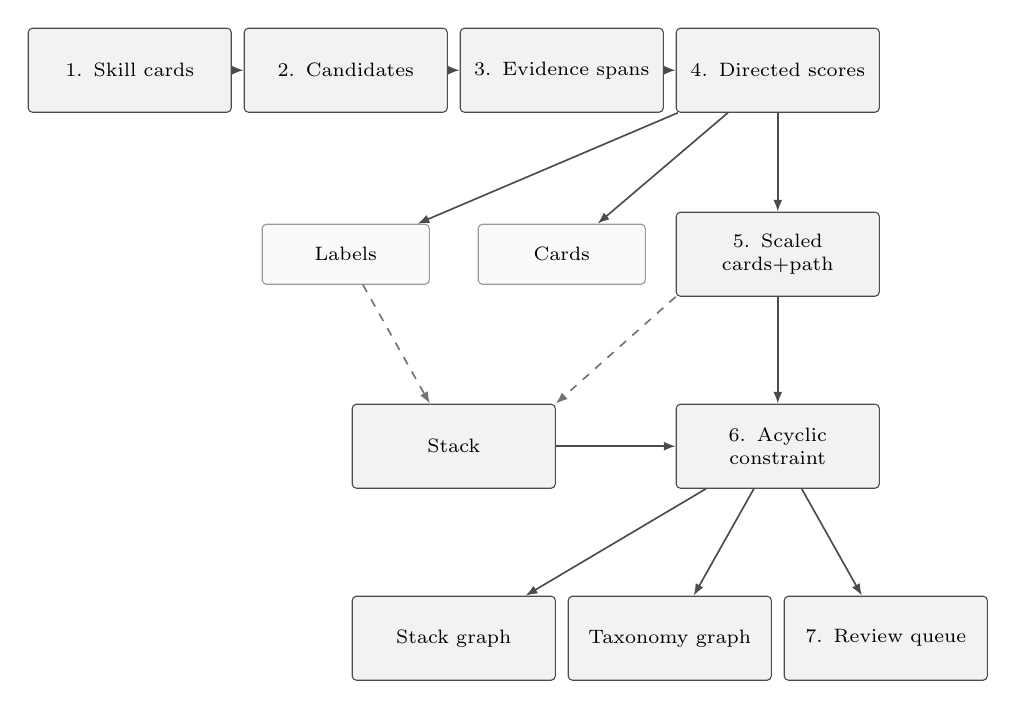
\begin{tikzpicture}[x=1in, y=1in,
  font=\scriptsize,
  box/.style={draw=black!70, rounded corners=1.5pt, align=center,
    text width=0.96in, minimum height=0.42in, inner sep=2pt,
    fill=black!5},
  stop/.style={draw=black!40, rounded corners=1.5pt, align=center,
    text width=0.78in, minimum height=0.30in, inner sep=2pt,
    fill=black!2},
  arr/.style={-{Latex[length=1.5mm]}, semithick, draw=black!70},
  darr/.style={-{Latex[length=1.5mm]}, semithick, draw=black!55, dashed}
]
\node[box] (s1) at (0.50, 0) {1. Skill cards};
\node[box] (s2) at (1.58, 0) {2. Candidates};
\node[box] (s3) at (2.66, 0) {3. Evidence spans};
\node[box] (s4) at (3.74, 0) {4. Directed scores};
\node[stop] (lab) at (1.58,-0.92) {Labels};
\node[stop] (card) at (2.66,-0.92) {Cards};
\node[box] (s5) at (3.74,-0.92) {5. Scaled cards$+$path};
\node[box] (stk) at (2.12,-1.88) {Stack};
\node[box] (s6) at (3.74,-1.88) {6. Acyclic constraint};
\node[box] (sg) at (2.12,-2.84) {Stack graph};
\node[box] (tg) at (3.20,-2.84) {Taxonomy graph};
\node[box] (s7) at (4.28,-2.84) {7. Review queue};
\draw[arr] (s1) -- (s2);
\draw[arr] (s2) -- (s3);
\draw[arr] (s3) -- (s4);
\draw[arr] (s4) -- (lab);
\draw[arr] (s4) -- (card);
\draw[arr] (s4) -- (s5);
\draw[darr] (lab) -- (stk);
\draw[darr] (s5.south west) -- (stk.north east);
\draw[arr] (stk) -- (s6);
\draw[arr] (s5) -- (s6);
\draw[arr] (s6) -- (sg);
\draw[arr] (s6) -- (tg);
\draw[arr] (s6) -- (s7);
\end{tikzpicture}
\caption{Seven-step data flow, with two graph branches.
Labels and Cards stop after the directed scores.
Cards$+$path is scaled, then constrained.
The stack combines the mention rule with the Labels and
Cards$+$path scores and enters the same acyclic step.
Dashed arrows mark those score inputs.}
\label{fig:pipeline}
\end{figure}

Table~\ref{tab:cond} names the comparisons.
In the scoring logs the three prompts are stored as B1, B3, and B5;
the reproduction note in \ref{app:repro} records that map.

\begin{table}[th]
\tbl{Conditions compared in the experiments.
The graph row transforms scores already
obtained; it does not call the model again.}
{\begin{tabular}{@{}lccc@{}}
\toprule
Condition & Prompt & Scaling & Graph \\
\colrule
Labels & label and description & no & no \\
Cards & same text as a retrieved span & no & no \\
Cards$+$path & span plus taxonomy path & no & no \\
Scaled cards$+$path & span plus taxonomy path & yes & no \\
Graph & span plus taxonomy path & yes & yes \\
Stack & mention, Labels, Cards$+$path & logistic & optional \\
\botrule
\end{tabular}}
\label{tab:cond}
\end{table}

\subsection{From scores to an acyclic graph}
\label{sec:alg}
Let $\tau$ be the operating threshold, let $\mu=0.8$, and let
$\delta=0.05$.
Self-loops are dropped.
If both directed probabilities exceed $\tau$ and differ by less
than $\delta$, the pair is marked as a direction conflict and both
values are kept.
Otherwise the weaker value is replaced by
$\min(\tilde{p}_{\mathrm{weak}},\max(0,\mu-\tilde{p}_{\mathrm{strong}}))$.
Edges with $\tilde{p}_{AB}\ge\tau$ enter the graph.
While a strongly connected component has more than one vertex, the
edge of lowest scaled confidence is deleted; ties break by source
identifier, then by target identifier.
A taxonomy flag records a high-confidence cross-branch pair
($\tilde{c}_{AB}>0.8$) and leaves the edge in place.
The type label that would separate a direct edge from a transitive
shortcut is defined so the schema is complete, and it is left unused
in the tables: annotators almost never chose it
(Section~\ref{sec:human}).
The quantity $\Lirr=\mathrm{mean}\max(0,\tilde{p}_{AB}+\tilde{p}_{BA}-\mu)$
on gold-positive pairs follows the irreversibility penalty of
{ProPRL}\cite{Cheng_2026} as a post-hoc summary, with no gradient
step.
Algorithm~\ref{alg:c23} states the procedure used for every reported
graph.
Batch sizes and deletion counts are in \ref{app:repro}.

\begin{algorithm}[t]
\caption{Reverse-conflict suppression and cycle breaking.}
\label{alg:c23}
\begin{algorithmic}[1]
\Require scored pairs; threshold $\tau$; margin $\mu$; band $\delta$
\For{each ordered pair $(A,B)$}
  \If{$A=B$}
    \State drop the pair
  \ElsIf{$\tilde{p}_{AB}>\tau$, $\tilde{p}_{BA}>\tau$, and $\lvert\tilde{p}_{AB}-\tilde{p}_{BA}\rvert<\delta$}
    \State mark a direction conflict and keep both values
  \Else
    \State replace the weaker value by $\min(\tilde{p}_{\mathrm{weak}},\max(0,\mu-\tilde{p}_{\mathrm{strong}}))$
  \EndIf
  \If{$\tilde{p}_{AB}\ge\tau$}
    \State accept $A\to B$
  \EndIf
\EndFor
\While{a strongly connected component has more than one vertex}
  \State delete its lowest-$\tilde{c}$ internal edge
\EndWhile
\State \Return the remaining edges
\end{algorithmic}
\end{algorithm}

\subsection{Which field each metric uses}
\label{sec:fields}
Verbalized confidence and the directed probability answer different
questions.
Confidence is a single number for the pair; the directed probability
is what the graph thresholds.
Table~\ref{tab:fields} is the map used throughout the results.
Pairwise ranking tables use verbalized confidence.
That field is the model's own certainty about the pair, and both
calibration and the pair-level threshold are defined on it.
The directed probability answers a different question, the chance of
one direction, and it is the field the graph thresholds.
On the taxonomy prompt the directed probability does rank the test
pairs better ({PR}-{AUC} $0.120$ against $0.101$ for confidence;
\ref{app:fields}).
The two fields still order those pairs in the same direction.
Cycle deletion follows scaled confidence, because that is the
uncertainty attached to the edge.
The acceptance decision follows the directed probability.

\begin{table}[th]
\tbl{Metric-to-field map.
Temperature scaling is monotone, so it leaves {ROC}-{AUC} and
{PR}-{AUC} unchanged and moves only thresholded {F1}.}
{\begin{tabular}{@{}ll@{}}
\toprule
Metric & Field \\
\colrule
{ROC}-{AUC}, {PR}-{AUC}, {F1} at $0.5$ & $\chat$ \\
{F1} at $\tau$ for Cards and Cards$+$path & $\tilde{c}$ \\
Direction accuracy & $\phat_{AB}$ against $\phat_{BA}$ \\
Edge acceptance & $\tilde{p}_{AB}$ \\
Cycle-deletion order & $\tilde{c}$ \\
{ECE}, {Brier} & $\chat$ and $\tilde{c}$ \\
Graph {F1} & $2\,\mathrm{TP}/(\lvert E\rvert+\lvert\mathrm{gold}\rvert)$ \\
\botrule
\end{tabular}}
\label{tab:fields}
\end{table}

Pair {ROC}-{AUC}, {PR}-{AUC}, and {F1} at $\tau$ on the test split
are reported with $95$\% bootstrap intervals from $1{,}000$ resamples
(seed $42$).
With a $2$\% positive rate, {PR}-{AUC} is the ranking summary we
emphasize.
Direction accuracy is computed only on gold edges oriented
$A\to B$.

\section{Experimental Setup}
\label{sec:setup}

\subsection{Data, split, and models}
The corpus is the public {ESCO-PrereqSkill} release\cite{Le_2025}.
After conversion there are 5,628 skills, 5,817 gold-edge records
($5{,}797$ unique directed pairs), and 5,627 cards.
One unresolved name has an identifier and no card.
The primary candidate pool contains $135{,}726$ directed pairs and
covers $2{,}800$ of the $5{,}797$ gold edges ($48.3$\%).
Split E follows Zhu and Zamani\cite{Zhu_2022}: any pair that touches
a held-out skill is reserved for test.
The training slice has $77{,}507$ pairs, validation has $8{,}611$
pairs, and the test slice has $49{,}608$ pairs with $1{,}003$
positives.
A closed split that reuses concepts is used only as a robustness
check in \ref{app:fields}.
\texttt{gpt-4o-mini} is the model used for every published graph.
{Qwen} 2.5 7B Instruct is scored on the same split as a second
family.
Both decoders use temperature $0$.
The prompts are in \ref{app:prompts}.

\subsection{Lexical baselines}
The mention rule fires when the source label occurs in the target
card.
{TF}-{IDF} cosine uses word and bigram features of the same card
text.
A linear {SVM} and a logistic regression are fit on the training
pairs of split E.
The stack used in the tables is a separate logistic regression on
three features of each directed pair: the mention indicator,
verbalized confidence from the labels prompt, and verbalized
confidence from the card-plus-path prompt.
Its coefficients are fit on the training pairs, and its threshold
is chosen on validation alone, on a grid of width $0.05$.
A mention-graph analogue of RefD, whose related set is the skills
mentioned in a card, reaches {PR}-{AUC} $0.141$.
This construction is a graph-level reformulation of the mention
rule, and the one-line rule remains stronger.
The shared-path orientation of the taxonomy prefix ranks below
chance ({AUC} $0.163$) because most skills sit at path length two
and gold edges often cross the top-level branches.
Reversing that orientation ranks above chance; precision--recall
stays at the base rate because of ties.

\subsection{Author-labeled sample}
\label{sec:human}
Two annotators and one adjudicator, the three authors, labeled 240
pairs on a four-way type and a direction.
They saw labels, descriptions, taxonomy paths, and retrieved spans,
and they did not see gold or model scores.
The sheet mixed an 80-pair overlap with pairs unique to each
annotator (seed $42$).
On the overlap, raw agreement is $0.875$ and Cohen's $\kappa$ is
$0.79$.
The adjudicated labels contain 58 direct pairs, 151 none, 31
ambiguous, and no transitive pair.
Binary metrics treat direct as positive.
A second sheet oversampled gold shortcuts and edges with an
alternate path.
Agreement there is $0.812$ ($\kappa=0.72$), and the transitive
label was used once.
The type field is therefore a schema slot rather than a measured
classifier.
Selective-review accuracy uses the first sheet only.

\section{Results}
\label{sec:results}

\subsection{RQ1: the card as evidence}
\label{sec:rq1}
Presenting the skill card as evidence improves ranking for
\texttt{gpt-4o-mini} and lowers direction accuracy
(Table~\ref{tab:rank}).
{ROC}-{AUC} rises from $0.834$ to $0.886$ and {PR}-{AUC} from
$0.085$ to $0.099$.
Adding the taxonomy path leaves both ranking metrics at the level
of the card prompt.
{F1} at the fixed cut $0.5$ falls because the card makes the model
attach edges densely (recall $0.98$ at precision $0.041$).
Under a $2$\% base rate that cut is a diagnostic.
The validation-chosen threshold $0.55$, applied to scaled
confidence, recovers {F1} $0.190$ for the card prompt and $0.203$
for the card-plus-path prompt.
A paired bootstrap of the card prompt against labels gives
$\Delta${ROC}-{AUC} $0.052$ ($0.043$--$0.062$) and
$\Delta${PR}-{AUC} $0.014$ ($0.009$--$0.020$), positive in all
$1{,}000$ resamples (Table~\ref{tab:ci}).
The {AUC} and {PR}-{AUC} intervals of the two evidence prompts
overlap, so the taxonomy path adds no further ranking gain.
Direction accuracy moves the other way: $0.761$ for labels, $0.667$
for cards, and $0.715$ once the path is restored.

A shuffled-card control separates the heading from the content.
On a gold-complete sample of the $1{,}003$ test positives and
$4{,}012$ random negatives, the matched card scores {ROC}-{AUC}
$0.887$.
A card taken from another pair scores $0.685$, below the
labels-only prompt on that sample ($0.836$).
The gain tracks the matched card.
The same format lowers ranking for {Qwen} 2.5 7B
(Section~\ref{sec:qwen}).

\begin{table}[th]
\tbl{Pair ranking on split E test ($49{,}608$ pairs, $1{,}003$
positives), \texttt{gpt-4o-mini}.
{AUC} and {PR}-{AUC} rank verbalized confidence.
{F1} at $\tau$ for the two evidence prompts uses the scaled value.
The stack row is fit on the training pairs; $\tau$ is chosen on
validation.}
{\begin{tabular}{@{}lcccccc@{}}
\toprule
Condition & F1@$0.5$ & F1@$\tau$ & $\tau$ & {AUC} & {PR}-{AUC} & {DA} \\
\colrule
Mention & $0.339$ & $0.339$ & $0.50$ & $0.620$ & $0.151$ & --- \\
{TF}-{IDF} & $0.044$ & --- & --- & $0.808$ & $0.070$ & --- \\
Jaccard & $0.005$ & --- & --- & $0.564$ & $0.027$ & --- \\
Labels & $0.163$ & $0.163$ & $0.50$ & $0.834$ & $0.085$ & $\mathbf{0.761}$ \\
Cards & $0.079$ & $0.190$ & $0.55$ & $\mathbf{0.886}$ & $0.099$ & $0.667$ \\
Cards$+$path & $0.071$ & $0.203$ & $0.55$ & $0.880$ & $0.101$ & $0.715$ \\
Stack & --- & $\mathbf{0.336}$ & $0.20$ & $0.898$ & $\mathbf{0.260}$ & --- \\
Linear {SVM} & $0.014$ & $0.111$ & $0.30$ & $0.697$ & $0.073$ & --- \\
\botrule
\end{tabular}}
\label{tab:rank}
\end{table}

\begin{table}[th]
\tbl{Bootstrap $95$\% intervals on split E test ($1{,}000$ resamples,
seed $42$) for the verbalized-confidence scores in
Table~\ref{tab:rank}.}
{\begin{tabular}{@{}lccc@{}}
\toprule
Condition & {AUC} & {PR}-{AUC} & F1@$\tau$ \\
\colrule
Mention & $[0.608,0.634]$ & $[0.130,0.175]$ & $[0.309,0.372]$ \\
Labels & $[0.820,0.846]$ & $[0.077,0.093]$ & $[0.152,0.175]$ \\
Cards & $[0.878,0.893]$ & $[0.092,0.108]$ & $[0.179,0.202]$ \\
Cards$+$path & $[0.872,0.888]$ & $[0.093,0.111]$ & $[0.190,0.217]$ \\
\botrule
\end{tabular}}
\label{tab:ci}
\end{table}

\subsection{RQ2: mention and the stack}
\label{sec:rq2}
The mention rule reaches {PR}-{AUC} $0.151$, above every standalone
model row in Table~\ref{tab:rank}.
{TF}-{IDF} is a strong {ROC} ranker and a weak precision--recall
ranker.
Neither the linear {SVM} nor class-weighted logistic regression
passes the mention rule.
A simple disjunction of mention and the taxonomy prompt at
$\tau=0.55$ improves recall ($0.616$) at the cost of precision
($0.126$).
The combination reported below is the train-fit stack defined in
Section~\ref{sec:setup}.
On the test split it reaches {ROC}-{AUC} $0.898$ and {PR}-{AUC}
$0.260$.
At its validation threshold ($\tau=0.20$) precision is $0.523$,
recall is $0.247$, and {F1} is $0.336$.
Mention {F1} at $0.5$ remains slightly higher ($0.339$), so the
stack wins on ranking rather than at every operating cut.
The model scores become useful for ranking once they are combined
with the lexical rule.
Pairs whose labels overlap lexically are scored highly even without
evidence; \ref{app:examples} shows four illustrative pairs.

\subsection{RQ3: two graphs}
\label{sec:rq3}
Structural constraints turn the scaled taxonomy-prompt scores into
one acyclic graph, and the same constraints turn the train-fit stack
into another (Table~\ref{tab:graph}).
The taxonomy graph keeps $8{,}896$ edges at precision $0.102$,
full-gold recall $0.157$, and graph {F1} $0.124$.
Before cycle breaking, the same scores keep $31{,}670$ directed
edges and recover more gold at lower precision.
Cycle breaking guarantees acyclicity at a substantial cost in
recall: test recall falls from $0.886$ to $0.344$ ($345$ of
$1{,}003$ gold test edges).
Direction accuracy on those $345$ edges is $0.554$, below the
score-level figure of $0.715$ on all gold test edges, because the
deleted edges are not a random subset.
The closure of the taxonomy graph reaches $1{,}220$ gold edges
($0.210$ of unique gold).
\ref{app:repro} records how many accepted edges also have an
alternate path.

The stack graph is the higher-precision output.
It keeps $1{,}334$ edges at precision $0.530$, full-gold recall
$0.122$, and graph {F1} $0.198$.
Recall on the original $1{,}003$ test gold edges is $0.245$ ($246$
edges), below the taxonomy graph.
Precision is about five times higher, and graph {F1} is higher.
An audit that prefers fewer false edges would take the stack graph;
an audit that prefers coverage would take the taxonomy graph.
On the stack, both the acceptance cut and the cycle order use the
logistic probability.
The primary pool still bounds every graph built only from it:
coverage is $48.3$\%, and the taxonomy graph reaches $0.325$ of the
gold edges inside the pool because cycle breaking deletes true
positives.
\ref{app:pool} reports the same constraints on a wider candidate
pool and on a graph that also includes the training pairs.

\begin{table}[th]
\tbl{Directed graphs on $5{,}797$ unique gold edges.
{F1} is full-gold graph {F1}.
The taxonomy rows threshold scaled $\tilde{p}_{AB}$ at $0.55$.
The stack row thresholds the train-fit logistic probability at
$0.20$.
R test uses the $1{,}003$ gold test edges.}
{\begin{tabular}{@{}lccccccc@{}}
\toprule
Graph & $\lvert E\rvert$ & Prec. & {F1} & R full & R pool & R val$+$test & R test \\
\colrule
Cards$+$path at $\tau$ & $31{,}670$ & $0.077$ & $0.131$ & $0.423$ & $0.875$ & $0.884$ & $0.886$ \\
Taxonomy graph & $8{,}896$ & $0.102$ & $0.124$ & $0.157$ & $0.325$ & $0.344$ & $0.344$ \\
Stack graph & $1{,}334$ & $0.530$ & $0.198$ & $0.122$ & $0.253$ & $0.238$ & $0.245$ \\
\botrule
\end{tabular}}
\label{tab:graph}
\end{table}

The threshold $\tau=0.55$ was fixed by maximizing pair-level {F1} of
scaled confidence on the validation split, before a graph {F1} was
computed.
Table~\ref{tab:sens} then rebuilds a graph from the validation pairs
alone ($192$ gold edges) across nearby thresholds.
At $\tau=0.60$, graph {F1} rises from $0.148$ to $0.242$ because
precision rises from $0.081$ to $0.165$ while recall falls from
$0.813$ to $0.453$, and the graph shrinks from $1{,}921$ edges to
$528$.
Pair {F1} and this graph {F1} select different operating points, and
$192$ gold edges are too few to replace the pair-level cut that
defines the published graphs.
Table~\ref{tab:sens} makes this trade-off explicit.
The margin $\mu\in\{0.6,0.8,1.0\}$ leaves every row unchanged: when
$\mu\le 1$ and $\tau\ge 0.5$, the weaker direction is always pushed
below $\tau$.
The $0.05$ band and the cross-branch flag mark pairs and do not
delete edges.

\begin{table}[th]
\tbl{Validation-only graphs from scaled Cards$+$path scores
($8{,}611$ pairs, $192$ gold edges, $\mu=0.8$).
The same edge counts appear at $\mu\in\{0.6,1.0\}$.
These graphs are a sensitivity display, separate from
Table~\ref{tab:graph}.}
{\begin{tabular}{@{}lcccc@{}}
\toprule
$\tau$ & $\lvert E\rvert$ & Prec. & Recall & {F1} \\
\colrule
$0.50$ & $2{,}623$ & $0.064$ & $0.875$ & $0.119$ \\
$0.55$ & $1{,}921$ & $0.081$ & $0.813$ & $0.148$ \\
$0.60$ & $528$ & $0.165$ & $0.453$ & $0.242$ \\
$0.70$ & $21$ & $0.048$ & $0.005$ & $0.009$ \\
\botrule
\end{tabular}}
\label{tab:sens}
\end{table}

\subsection{Calibration}
\label{sec:cal}
Temperature scaling barely moves expected calibration error on the
taxonomy prompt, from $0.306$ to $0.299$ (Table~\ref{tab:cal}).
The map divides the logit by a temperature and has no intercept, so
it cannot remove a systematic over-positive bias at a $2$\% base
rate.
Platt scaling and a three-parameter beta map drive {ECE} to about
$0.001$ by sending almost every score to that base rate.
Because those maps are monotone, a threshold rechosen on validation
would leave pair {F1} and {AUC} unchanged.
They are poor graph-stage maps: Algorithm~\ref{alg:c23} compares
scores with absolute constants, and a map that collapses to the base
rate makes those constants meaningless.
The {JSON} values are discrete in steps of $0.1$, so many pairs
share a rank.
That granularity affects calibration error and the order of cycle
deletion.

\begin{table}[th]
\tbl{Calibration on split E test.
Temperature is fit on validation.
{ECE} and {Brier} use verbalized confidence, raw and scaled.}
{\begin{tabular}{@{}lcccc@{}}
\toprule
Condition & $T$ & {ECE} raw & {ECE} scaled & {Brier} raw / scaled \\
\colrule
Labels & $3.2$ & $\mathbf{0.086}$ & $0.109$ & $0.055$ / $0.064$ \\
Cards & $3.9$ & $0.282$ & $0.273$ & $0.174$ / $0.146$ \\
Cards$+$path & $3.3$ & $0.306$ & $0.299$ & $0.178$ / $0.160$ \\
\botrule
\end{tabular}}
\label{tab:cal}
\end{table}

\subsection{A second model family}
\label{sec:qwen}
The card effect reverses on {Qwen} 2.5 7B (Table~\ref{tab:qwen}).
On the test split, {ROC}-{AUC} falls from $0.803$ for labels to
$0.654$ for cards; the taxonomy path recovers part of the drop
($0.696$) and remains below labels.
{PR}-{AUC} follows the same order, while direction accuracy rises.
Validation shows the same pattern.
Whether a taxonomy card helps ranking therefore depends on the
model.
The comparison confounds model family with model size: one system
is a proprietary model and the other is an open 7B model.
A separate {Qwen}3 27B pass on the validation pairs, unused in any
graph, ranks by the directed probability at {AUC} $0.711$ and by
verbalized confidence at {AUC} $0.202$.
An inverted confidence field would change which edges cycle breaking
removes, which is why that pass stays out of Algorithm~\ref{alg:c23}.
On \texttt{gpt-4o-mini} the same confidence field has {AUC} $0.880$
(\ref{app:fields}).

\begin{table}[th]
\tbl{{Qwen} 2.5 7B.
{F1} is at $0.5$.
{AUC} and {PR}-{AUC} rank verbalized confidence.
Direction accuracy compares the two directed probabilities.}
{\begin{tabular}{@{}lccccc@{}}
\toprule
Condition & Split & F1@$0.5$ & {AUC} & {PR}-{AUC} & {DA} \\
\colrule
Labels & validation & $0.067$ & $\mathbf{0.814}$ & $\mathbf{0.080}$ & $0.839$ \\
Cards & validation & $0.045$ & $0.652$ & $0.034$ & $0.901$ \\
Cards$+$path & validation & $0.044$ & $0.710$ & $0.042$ & $\mathbf{0.943}$ \\
Labels & test & $\mathbf{0.061}$ & $\mathbf{0.803}$ & $\mathbf{0.062}$ & $0.809$ \\
Cards & test & $0.041$ & $0.654$ & $0.032$ & $0.908$ \\
Cards$+$path & test & $0.040$ & $0.696$ & $0.036$ & $\mathbf{0.947}$ \\
\botrule
\end{tabular}}
\label{tab:qwen}
\end{table}

\subsection{Author labels}
On the 240 author labels, uncertainty sampling at a ten-percent
budget (24 pairs) reaches accuracy $0.808$, against $0.796$ for a
random slice of the same size.
The bootstrap interval on that gap includes zero.
At twenty and thirty percent the gaps are $+0.054$
($0.017$--$0.092$) and $+0.067$ ($0.021$--$0.096$).
Those intervals exclude zero, so on this author-labeled sample
uncertainty sampling shows a small positive signal.
The comparison was specified after the labels existed, and the
annotators had seen the retrieved spans.
Table~\ref{tab:human} compares the same scores with the 240 labels.
The slice is denser in positives than the ontology, and it agrees
with the ranking pattern of \texttt{gpt-4o-mini} on split E.

\begin{table}[th]
\tbl{The 240 author-labeled pairs.
Positive means direct; none and ambiguous count as negative.}
{\begin{tabular}{@{}lcccc@{}}
\toprule
Condition & F1@$0.5$ & F1@$0.55$ & {AUC} & {PR}-{AUC} \\
\colrule
\texttt{gpt-4o-mini} Labels & $\mathbf{0.714}$ & $\mathbf{0.768}$ & $0.872$ & $0.634$ \\
\texttt{gpt-4o-mini} Cards & $0.435$ & $0.641$ & $0.899$ & $0.612$ \\
\texttt{gpt-4o-mini} Cards$+$path & $0.494$ & $0.699$ & $\mathbf{0.949}$ & $\mathbf{0.748}$ \\
{Qwen} 2.5 7B Cards & $0.395$ & $0.459$ & $0.720$ & $0.550$ \\
\botrule
\end{tabular}}
\label{tab:human}
\end{table}

\section{Discussion}
\label{sec:discussion}
The card effect splits by model.
For \texttt{gpt-4o-mini}, restating the skill's own card under an
evidence heading improves ranking, and a card drawn from another
pair removes that gain.
For {Qwen} 2.5 7B the same restatement lowers ranking on both
validation and test.
Work on verbalized confidence finds that the number a model writes
down is sensitive to the prompt and is often
over-confident\cite{Tian_2023,Xiong_2024}.
A reading consistent with that evidence is that the two models use
a prompted evidence block differently: one treats the matched card
as support, and the other lets the repeated text inflate both
directions.
Because only the verbalized outputs were recorded,
instruction-following effects cannot be separated from
context-length effects.
Direction accuracy and ranking move in opposite directions for both
models, so a prompt that helps one of them can hurt the other.

On this release the lexical rule is the strong prior.
Gold edges often pair a knowledge label with an action that repeats
it, which is why mention reaches a higher standalone {PR}-{AUC}
than any single prompt.
The language model still recovers gold edges the rule misses, and
the stack is the way those two signals combine.
{LECDPR}\cite{Xiao_2026} invests the retrieved text in a graph
neural network over concept--document interactions.
{ProPRL}\cite{Cheng_2026} trains against bidirectional
over-confidence; Algorithm~\ref{alg:c23} applies a related penalty
only at inference, after the scores exist.
Le and Abel\cite{Le_2025} generate prerequisite names and align
them.
The tool here scores directed pairs inside a fixed candidate pool
and returns an edge with a span.
These systems address different tasks, and their {F1} tables answer
different questions.

For a practitioner the choice is between the two graphs in
Table~\ref{tab:graph}.
The stack graph is the output to hand to an audit that prefers
fewer false edges.
The taxonomy graph is the output when missing a gold edge is more
costly than an extra edge, with the understanding that cycle
breaking has already removed many true positives.
Both graphs are bounded by candidate generation.
A pool that also kept single-token label overlap would cover
$74.9$\% of gold edges, at the cost of a substantially larger
candidate set (about $562$k pairs).

The result is tied to {ESCO} cards under an unseen-concept split.
Extending either model to lecture slides, Wikipedia lead sections,
or a taxonomy whose gold edges are less lexical requires a second
corpus.
External raters who have not seen the retrieved spans would be
needed before the human sample could support a selective-review
policy.

\section{Limitations}
\label{sec:limit}
The primary pool contains fewer than half of the gold edges, so a
perfect classifier on that pool would still miss most of the
ontology.
Wikipedia sitelinks and lecture slides are too sparse, or too
incomplete in the public files, to serve as a second corpus.
The human sample was labeled by the authors after they had seen
retrieved spans, and the transitive type was almost never chosen, so
the type field remains unchecked.
A slice of skills introduced after the model cutoff is not
available: the identifier difference against {ESCO} v1.1.1 contains
no gold positive in the test split.
Label permutation drives {AUC} to chance
(\ref{app:fields}), which shows that the metrics respond
to label structure.
The two scored models differ in both family and size, so the card
effect cannot yet be attributed to family alone.
The two graphs use thresholds chosen on validation for pair {F1}.
Table~\ref{tab:sens} shows that a different objective, graph {F1} on
$192$ validation gold edges, prefers a sparser cut.

\section{Conclusion}
\label{sec:conclusion}
Restating a skill card as evidence improves pairwise ranking for
\texttt{gpt-4o-mini} and lowers it for {Qwen} 2.5 7B, and it lowers
direction accuracy for the first model.
A mention rule is the stronger standalone ranker; stacking it with
the model scores is what makes those scores useful.
Temperature scaling leaves calibration almost unchanged and is kept
because the graph constraints use absolute cuts.
The resulting taxonomy graph recovers more gold edges, and the stack
graph is more precise.
The next useful measurement is a second corpus whose documents are
not the skill cards themselves, scored with the same metric-to-field
map.

\section*{Data and Code Availability}
{ESCO-PrereqSkill} is public\cite{Le_2025}.
A reproduction pack contains the conversion and scoring scripts, the
prompts, the configuration (seed $42$, unseen-concept fraction
$0.2$), the held-out skill identifiers, the two 240-pair human
sheets, and the pair scores needed to recompute the test tables.
The pack is public at
\url{https://github.com/tuanymc/p2a-prerequisite-graphs}.
The full prompt-and-span logs will be posted with the camera-ready
version.

\section*{Conflict of Interest}
The authors declare that they have no conflict of interest.

\section*{Funding}
This work received no specific grant from any funding agency.

\section*{ORCID}
Thu Do Thi --- \url{https://orcid.org/0009-0007-0220-3847}

\noindent Tuan Dao Minh --- \url{https://orcid.org/0009-0009-1641-6813}

\noindent Anh-Hien Dao --- \url{https://orcid.org/0009-0000-9619-1603}

\appendix
\section{Scoring Prompts}
\label{app:prompts}
The system message is shared by the three prompts:
\begin{verbatim}
You judge directed prerequisite relations.
Return JSON only. Do not invent quotations.
Cite only provided evidence_ids.
Fields:
- p_A_to_B, p_B_to_A: numeric floats in [0,1],
  never strings or labels
- relation_type: direct | transitive | none | ambiguous
- direction: A_to_B | B_to_A | none
- confidence_raw: numeric float in [0,1]
- rationale: short string
- evidence_ids: array of provided ids
\end{verbatim}
The user message begins with the two skill records.
Cards$+$path then inserts \texttt{Taxonomy A:} and
\texttt{Taxonomy B:}.
Cards and Cards$+$path append retrieved windows as
\texttt{Evidence A$\to$B:} and \texttt{Evidence B$\to$A:}.
Labels replaces those blocks with ``No retrieved evidence.
Do not fabricate spans.''
In the released logs, Labels, Cards, and Cards$+$path are the
conditions B1, B3, and B5.
The directed probabilities are $\phat_{AB}$ and $\phat_{BA}$.
The verbalized confidence is $\chat_{AB}$.

\section{Reproduction Notes}
\label{app:repro}
On the reported full-pool run, reverse-conflict suppression flags
$10{,}699$ of the $31{,}670$ edges that pass $\tau=0.55$.
Cycle breaking then deletes $22{,}774$ edges and leaves the
$8{,}896$-edge graph.
The batched pass deletes $21{,}375$ edges; a sequential cleanup
deletes the remaining $1{,}399$ over $153$ rounds.
When several edges in one component share a confidence, the deleted
edge is the one with the smaller source identifier, then the smaller
target identifier.
A cross-branch flag marks $178$ high-confidence pairs and deletes
none.
Every scored pair has a card window, so the missing-evidence flag
is never raised.
Of $7{,}985$ accepted edges that miss a direct gold link, four lie
on the gold transitive closure.
Of the accepted edges, $16.7$\% have an alternate path, and $173$
of those paths are gold-direct.
A transitive reduction of the gold graph finds $38$ shortcuts
($0.7$\% of $5{,}797$).
The second author sheet assigned \texttt{transitive} once, so that
type stays unevaluated as a classifier.

\section{Score Fields and Robustness}
\label{app:fields}
On the $49{,}608$ test pairs, verbalized confidence for the
taxonomy prompt has {ROC}-{AUC} $0.880$ and {PR}-{AUC} $0.101$,
which are the Cards$+$path entries in Table~\ref{tab:rank}.
The directed probability on the same rows has {ROC}-{AUC} $0.894$
and {PR}-{AUC} $0.120$.
The rank correlation of the two fields is $0.880$.
Thresholding the scaled directed probability at $0.55$ gives pair
{F1} $0.143$ (precision $0.078$, recall $0.887$).
That cut is the pair-level form of edge acceptance.
Labels and Cards show the same pattern: confidence matches
Table~\ref{tab:rank} ({AUC} $0.834$ and $0.886$), while the directed
probability has {AUC} $0.859$ and $0.885$.
Cycle deletion on the taxonomy graph follows scaled confidence.
Replacing that order with the directed probability would define a
different graph; \ref{app:repro} describes the reported graph.

Labels {F1} is $0.163$ on split E and $0.156$ on the closed split A.
A zero-shot scorer has no weights for the split to change.
Permuting the test labels (20 shuffles, seed $42$) drops {ROC}-{AUC}
to $0.50$ (interval $0.49$--$0.51$) and {PR}-{AUC} to the $2$\% base
rate for labels, cards, the taxonomy prompt, and mention.
This permutation test confirms that the metrics are sensitive to
label structure; it does not, however, establish whether the model
memorized {ESCO}.
{ESCO} v1.2 (May 2024) is after the October 2023 knowledge cutoff of
\texttt{gpt-4o-mini}.
The identifier difference against the September 2022 public list
yields one new skill, ten test pairs, and zero gold positives.

\section{Illustrative Pairs}
\label{app:examples}
These examples are illustrative and were not sampled to be
representative.
Values are $\phat_{AB}/\phat_{BA}$.
\emph{Soldering techniques} before \emph{apply soldering techniques}
is $0.8/0.8$ under Labels and only slightly higher once the card is
shown, with both directions high.
\emph{Types of concrete pumps} before \emph{install concrete pumps}
moves from $0.0/0.0$ to $0.7/0.5$.
The same spans raise a same-verb distractor, \emph{assemble
mechatronic units} before \emph{assemble hardware components}, from
$0.3/0.2$ to $0.7/0.5$, and they raise both directions on a
gold-reverse pair, \emph{design user interface} before \emph{use
methodologies for user-centered design}.
An automatic audit of gold edges absent from the primary pool finds
no remaining edge whose one label is a token-subset of the other,
$22$ missed edges that share a bigram, and $1{,}548$ missed edges
with at least one shared token.

\section{Candidate-Pool Expansion}
\label{app:pool}
{TF}-{IDF} top-16 neighbors of the card text cover $3{,}636$ unique
gold edges ($0.627$).
The union with the primary pool covers $3{,}956$ ($0.682$).
The $63{,}718$ new pairs were scored once with the taxonomy prompt
(\texttt{gpt-4o-mini}, temperature $0$, zero errors).
Each pool then passes separately through Algorithm~\ref{alg:c23}.
Table~\ref{tab:expand} reports the three acyclic graphs.
We expected full-gold recall to rise by less than $0.02$, or the
interval to include zero.
Both pools rise by about $0.03$, and the intervals exclude zero.
On the original $1{,}003$ test gold edges the primary graph keeps
$345$, the neighborhood graph keeps $300$, and the union keeps
$309$.
Because the neighborhood omits some primary-pool pairs, the
pre-cycle edge set already falls from $889$ to $802$ true positives,
and cycle breaking leaves $300$.
The union keeps all $889$, then cycle breaking removes $36$ edges
the primary graph had kept.
Of the $172$ additional full-gold true positives in the neighborhood
graph, $56$ lie in an expanded test set of $1{,}425$ edges and $116$
lie in training or validation gold.
The primary pool contains none of the $422$ newly added test gold
edges, so those edges count against it before the classifier runs.
A top-32 neighborhood was left unscored; top-16 already shows the
recall gain and the cost on the original test gold.
Including the training pairs in the taxonomy graph raises full-gold
recall relative to a graph built only on validation and test, and
cycle breaking on that denser graph lowers test recall from $0.423$
to $0.344$.

\begin{table}[th]
\tbl{Full-gold recovery after scoring the {TF}-{IDF} top-16 pairs
absent from the primary pool ($5{,}797$ unique gold).
R original is recall on the $1{,}003$ gold test edges already inside
the primary pool.
Intervals are paired bootstrap percentiles, $1{,}000$ resamples,
seed $42$.}
{\begin{tabular}{@{}lccccccc@{}}
\toprule
Pool & $\lvert E\rvert$ & Prec. & {F1} & R full & R original & $\Delta$R & 95\% interval \\
\colrule
Primary & $8{,}896$ & $0.102$ & $0.124$ & $0.157$ & $0.344$ & $0$ & --- \\
{TF}-{IDF}-16 & $9{,}633$ & $0.112$ & $0.140$ & $0.187$ & $0.299$ & $+0.030$ & $0.022$--$0.037$ \\
Union & $10{,}325$ & $0.104$ & $0.133$ & $0.185$ & $0.308$ & $+0.028$ & $0.021$--$0.035$ \\
\botrule
\end{tabular}}
\label{tab:expand}
\end{table}

\section{Recovered Slices}
\label{app:slices}
On $4{,}640$ pairs recovered by single-token overlap outside the
primary pool ($1{,}544$ gold, positive rate $0.333$), repeating the
card raises \texttt{gpt-4o-mini} {ROC}-{AUC} by $0.127$
($0.115$--$0.138$) and {PR}-{AUC} by $0.110$ ($0.093$--$0.127$).
On {Qwen} 2.5 7B the same change lowers {ROC}-{AUC} by $0.058$
($0.048$--$0.067$) and {PR}-{AUC} by $0.117$ ($0.099$--$0.132$).
The interaction, the {Qwen} change minus the \texttt{gpt-4o-mini}
change, is $-0.184$ on {ROC}-{AUC} ($-0.200$ to $-0.169$) and
$-0.226$ on {PR}-{AUC} ($-0.251$ to $-0.205$).
These slices are denser than Table~\ref{tab:rank}.
Inside the {TF}-{IDF} top-16 neighbors ($3{,}468$ pairs, $1{,}156$
gold, the same positive rate) the card raises \texttt{gpt-4o-mini}
{ROC}-{AUC} by $0.048$ ($0.035$--$0.060$) and leaves {PR}-{AUC}
unchanged ($-0.001$; the interval includes zero), while it lowers
{Qwen} on both ({ROC} $-0.070$, {PR} $-0.078$).
The top-32 neighbor slice has the same signs.

\section{Token Cost}
\label{app:cost}
A 400-pair sample of taxonomy-prompt inputs for \texttt{gpt-4o-mini}
averaged $401$ input tokens (90th percentile $448$).
We budget $160$ output tokens.
At the October 2026 list price of \$0.15 / \$0.60 per million input
and output tokens, the validation-plus-test pass ($58{,}219$ pairs)
is about \$9, and the additional $77{,}507$ training pairs are about
\$12.
The {TF}-{IDF} expansion ($63{,}718$ pairs) is about \$10.
Labels on the training pairs and the new pairs ($141{,}225$ calls,
zero errors) is about \$22 on the same budget.
{Qwen} token bills were not retained.
Wall-clock time for the parallel score loop was about $3.8$~h
(labels), $5$~h (cards), $4.8$~h (taxonomy prompt, validation and
test), and $6.9$~h (taxonomy prompt, training).

\bibliographystyle{ws-ijait}
\bibliography{refs}

\end{document}
